\section{Quelle représentation ?}

\begin{multicols}{2}
	Tous les atomes de ce bijou possèdent 78 protons. 33\% d'entre eux possèdent 116 neutrons, 34\% 117 neutrons, 25 \% 118 et 7\% 120 neutrons.

	
	\begin{center}
		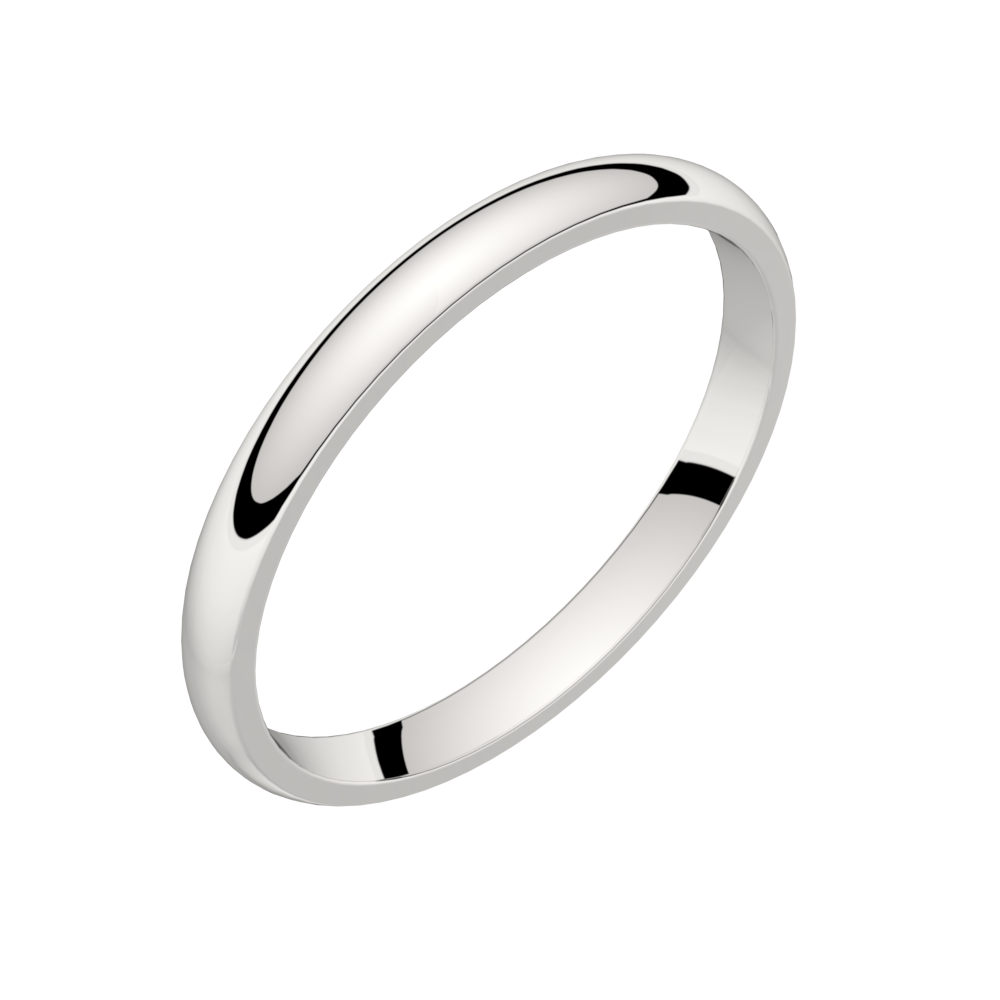
\includegraphics[scale=0.12]{img/ring2}
	\end{center}
\end{multicols}


\begin{questions}
	\question[1] De quels atomes le bijou est-il composé ?
	\fillwithdottedlines{2cm}
	\begin{solution}
		Les atomes de ce bijou possèdent tous 78 protons, ce sont donc des atomes de l'élément chimique de numéro atomique 78, le platine.
	\end{solution}
	
	\question[1] Comment appelle-t-on des atomes d'un même élément qui possèdent un nombre de neutrons différent ?
	\fillwithdottedlines{2cm}
	\begin{solution}
		Les isotopes sont des atomes d'un même élément qui possèdent un nombre de neutrons différent.
	\end{solution}
	
	\question[1] Préciser, en le justifiant le nombre d'électrons de ces atomes.
	\fillwithdottedlines{3cm}
	\begin{solution}
		Dans un atome il y a autant d'électrons que de protons, donc ces atomes possèdent 78 électrons. 
	\end{solution}
\end{questions}
